%from ChaosBook.org \Chapter{flows}{27aug2008}{Go with the flow}
% $Author: predrag $ $Date: 2009-02-22 13:26:43 -0500 (Sun, 22 Feb 2009) $
    %
%%%%%%%%%%%%%%%%%%%%%%%%%%%%%%%%%%%%%%%%%%%%%%%%%%%%%
\SFIG{lorenz_less_ugly_bm}{}
{Lorenz ``butterfly'' strange attractor.  (J. Halcrow)}
{LorenzAttrct}
%%%%%%%%%%%%%%%%%%%%%%%%%%%%%%%%%%%%%%%%%%%%%%%%%%%%%

%%%%%%%%%%%%%%%%%%%%%%%%%%%%%%%%%%%%%%%%%%%%%%%%%%%%%%%%%%%%%%%%%%%%%%%%%%
\example{Lorenz strange attractor:}{ \label{exmp:Lorenz}
% Predrag                           17feb2008
% Predrag                           10dec2007
% Predrag                           20sep2007
% transferred from halcrow/blog/TEX/lorenz.tex
Edward Lorenz arrived at the equation
\index{Lorenz flow}\index{Rayleigh-Benard flow}
\beq
\dot{\ssp}=\pVeloc(\ssp)
    =
    \left[
        \begin{array}{c}
\dot{x} \\ \dot{y} \\ \dot{z}
    \end{array}
    \right]
    =
    \left[
        \begin{array}{c}
\sigma (y-x) \\
\rho x - y -xz \\
xy -bz
    \end{array}
    \right]
\ee{Lorenz}
by a drastic simplification of
the Rayleigh-Benard flow. %\rf{lorenz63}.
Lorenz fixed
$\sigma = 10$, $ b= 8/3$,
and varied the ``Rayleigh number'' $\rho$. For
$0 < \rho < 1$ the \eqv\ $\EQV{0} =(0,0,0)$
at the origin is attractive.
At $ \rho = 1$  it undergoes a pitchfork
bifurcation into a pair of \eqva\ at
\index{equilibrium!Lorenz flow}
\beq
\ssp_{\EQV{1,2}} = (\pm \sqrt{b(\rho-1)}, \pm \sqrt{b(\rho-1)}, \rho-1)
\,,
\ee{LorEqva}
We shall not explore the Lorenz flow dependence on the $\rho$
parameter in what follows, but here is a brief synopsis: the
$\EQV{0}$  $1$\dmn\ unstable manifold closes into a
homoclinic orbit at $\rho=13.56\dots$. Beyond that, an infinity
of associated \po s are generated, until $\rho = 24.74\dots$,
where $\EQV{1,2}$ undergo a Hopf bifurcation.

All computations that follow
will be performed for the Lorenz parameter choice
\(
    \sigma = 10, b= 8/3, \rho = 28
\,.
\)
For these parameter values the long-time dynamics is confined to
the strange attractor
depicted in  \reffig{LorenzAttrct}.
(continued in \refexam{exmp:LorenzSect}.)
    \PC{ \reffig{LorenzAttrct} .eps still too big}
    } %end \example{Lorenz

%from ChaosBook.org \Chapter{maps}{13jun2008}{Discrete time dynamics}
% $Author: predrag $ $Date: 2009-02-22 13:26:43 -0500 (Sun, 22 Feb 2009) $


%%%%%%%%%%%%%%%%%%%%%%%%%%%%%%%%%%%%%%%%%%%%%%%%%%%%%%%%%%%%%%%%%%%%%%%%%%
\example{Sections of Lorenz flow:}{ \label{exmp:LorenzSect}
% Predrag                           04apr2008
% Predrag                           19jan2008
% moved to here from halcrow/blog/TEX/lorenz.tex
%%%%%%%%%%%%%%%%%%%%%%%%%%%%%%%%%%%%%%%%%%%%%%%%%%%%%
%
\FIG{{
(a)~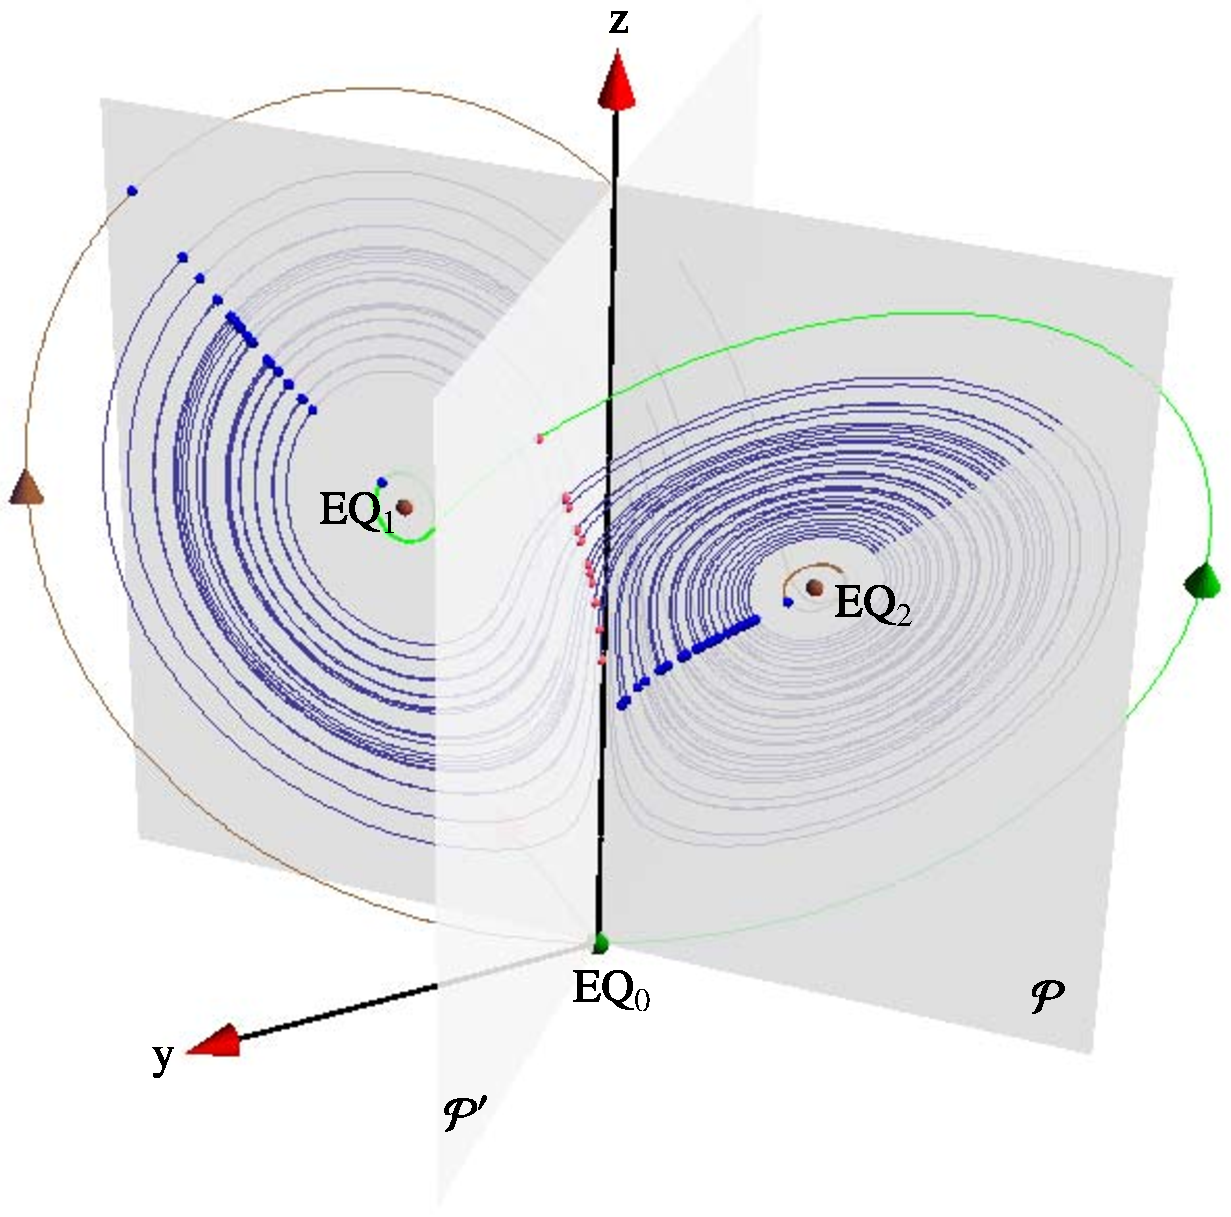
\includegraphics[width=0.48\textwidth]{../Fig/lorenz2Poinc}
(b)~\raisebox{1.0ex}{
    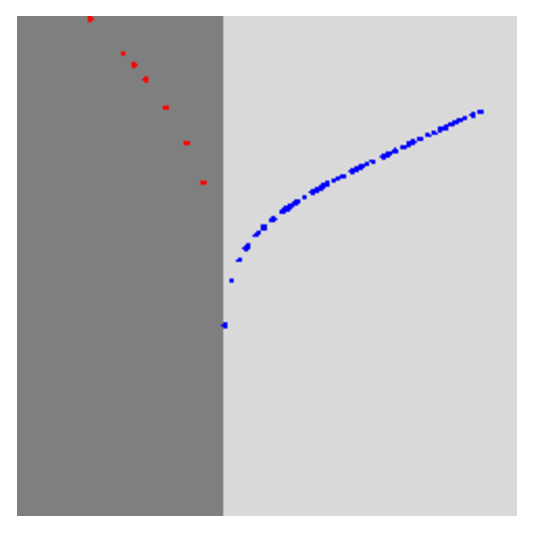
\includegraphics[width=0.30\textwidth]{../Fig/lorenz2Poinc2D}
                    }}
}{}{
(a) Lorenz flow \reffig{LorenzAttrct}
cut by  $y=x$ Poincar\'e section plane $\PoincS$
through the $z$ axis and both $\EQV{1,2}$ \eqva.
Points where flow pierces into section % $\PoincS$
are marked by dots.
To aid visualization of the flow near the $\EQV{0}$ \eqv,
the flow is cut by the second Poincar\'e section,  $\PoincS'$,
through $y=-x$ and the $z$ axis.
% Marking the ingoing sections yields a symmetric image.
(b) Poincar\'e sections $\PoincS$ and $\PoincS'$ laid side-by-side.
The singular nature of these sections close to $\EQV{0}$ will be
elucidated in \refexam{exmp:LorenzStab}
and \reffig{fig:PoincLorenz}\,(b).
(E. Siminos)
%       \(\sigma = 10, b= 8/3, \rho = 28\,.\)
}{fig:LorenzSect}
%%%%%%%%%%%%%%%%%%%%%%%%%%%%%%%%%%%%%%%%%%%%%%%%%%%%%
    %
\index{Lorenz flow}
%\PC{ChaosBook: an example in maps.tex chapter,
%    immediately after R\"ossler.}
(continued from \refexam{exmp:Lorenz}.)
The plane $\PoincS$
fixed by the $x=y$ diagonal and
the $z$-axis depicted in \reffig{fig:LorenzSect} is
a natural choice of a Poincar\'e section of the Lorenz
flow of \reffig{LorenzAttrct},
as it contains all three  \eqva, $\ssp_{\EQV{0}} =(0,0,0)$
and the \refeq{LorEqva} pair $\EQV{1,2}$.
A section has
to be supplemented with the orientation
condition \refeq{orientCond}: here
points where flow pierces \emph{into} the section
are marked by dots.
\index{equilibrium!Lorenz flow}

    \PC{\reffig{fig:LorenzSect}\,(b): generate
        .eps from lorenz2Poinc2D.pdf,
        this is the old version. Raise it a bit.
        }
$\EQV{1,2}$ are centers of out-spirals, and close to them  the
section % $\PoincS$ is transverse to the flow. However, close
to  $\EQV{0}$ trajectories pass the $z$-axis either by crossing
the section $\PoincS$ or staying on the viewer's side. We are
free to deploy as many sections as we wish: in order to capture
the whole flow in this neighborhood we add the second
Poincar\'e section, $\PoincS'$, through the $y=-x$ diagonal and
the $z$-axis. Together the two sections,
\reffig{fig:LorenzSect}\,(b), capture the whole flow near
$\EQV{0}$. In contrast to R\"ossler sections of
\reffig{f:RoeslSect}, these appear very singular. We explain
this singularity in \refexam{exmp:LorenzStab}, and postpone
construction of a Poincar\'e return map to
\refexam{exmp:LorenzD1}.
\hfill   (E. Siminos and J. Halcrow)
    } %end \example{exmp:LorenzSect


%from ChaosBook.org \Chapter{stability}{21feb2009}{Local stability}
% $Author: predrag $ $Date: 2009-02-22 13:26:43 -0500 (Sun, 22 Feb 2009) $
by the flow, \reffig{f:shear}.

\example{Lorenz flow, linearized:}{ \label{exmp:RossLinrz}
For the  Lorenz
\refeq{Lorenz} flow the {\stabmat} is
  \beq
{\Mvar_{Ross}} =
  \left(\barr{ccc}
    0  & -1 & -1 \\
    1  &  a &  0 \\
    z  &  0 & x-c
    \earr\right)
  \,.
  \ee{RossLinrz}
    }% end \example{R\"ossler...

%%%%%%%%%%%%%%%%%%%%%%%%%%%%%%%%%%%%%%%%%%%%%%%%%%%%%%%%%%%%%%%%%%%%%%%%%%
\example{Stability of Lorenz flow \eqva:}{ \label{exmp:LorenzStab}
% Predrag                           04apr2008
% Predrag                           19jan2008
% moved to here from halcrow/blog/TEX/lorenz.tex
%
\index{Lorenz flow}
(continued from \refexam{exmp:RossLinrz}.)~~
A glance at \reffig{fig:LorenzSect} suggests that the
flow is organized by its 3 \eqva, so lets have a closer look at
their stable/unstable manifolds.

\PC{ChaosBook: add pointer}
The $\EQV{0}$ \eqv\  {\stabmat} \refeq{RossLinrz}
evaluated at $\ssp_{\EQV{0}} =(0,0,0)$ is block-diagonal.
The $z$-axis is an eigen\-vector
with a contracting eigenvalue $\eigExp[2]=-b$.
From \refeq{trA-Lorenz} it follows that all $[x,y]$ areas
shrink at rate $-(\sigma +1)$. Indeed, the
$[x,y]$ submatrix
\beq
{\Mvar^{-}} =
  \left(\barr{cc}
    -\sigma  & \sigma  \\
    \rho     &   -1
    \earr\right)
\ee{LorzEQ0plus}
has a real expanding/contracting eigenvalue pair
$\eigExp[1,3]=
-(\sigma +1)/2 \pm \sqrt{(\sigma-1)^2/4 + \rho \sigma}$,
with the right eigen\-vectors $\jEigvec[1]$,  $\jEigvec[3]$
in the $[x,y]$ plane, given by (either) column of
the projection operator
\PC{ChaosBook: give refeq here}
\beq
{\PP_i} = \frac{\Mvar^{-} -\eigExp[j] \matId}{\eigExp[{i}]-\eigExp[{j}]}
 = \frac{1}{\eigExp[{i}]-\eigExp[{j}]}
  \left(\barr{cc}
    -\sigma  - \eigExp[{j}] & \sigma  \\
                 \rho   &   -1-\eigExp[{j}]
    \earr\right)
  \,,\qquad i \neq j \in \{1,3\}
  \,.
\ee{LorzEQ0eVect}


$\EQV{1,2}$ \eqva\ have no symmetry, so
their eigenvalues are given by
the roots of a cubic equation, the secular determinant
$\det(\Mvar - \Lyap  \matId)=0$:
\beq
% \EQV{0}~~ &:& \;\; (\eigExp[+],\Lyap_-,\Lyap_s)
%    =  (-(\sigma +1)/2 \pm \sqrt{(\sigma-1)^2/4 + \rho \sigma}, -b)
% \EQV{1,2} &:&  \;\;   \mbox{}
     \Lyap^3+\Lyap^2(\sigma+b+1)+\Lyap b(\sigma+\rho)+2\sigma b (\rho-1) = 0
\,.
\label{LorenzEqQigs}
\eeq
For $\rho > 24.74$, $\EQV{1,2}$ have one stable real eigenvalue and
one unstable complex conjugate pair, % as solutions to \refeq{LorenzEqQigs},
leading to a spiral-out instability and the strange attractor
depicted in  \reffig{LorenzAttrct}.


%%%%%%%%%%%%%%%%%%%%%%%%%%%%%%%%%%%%%%%%%%%%%%%%%%%%%
\FIG{
(a)  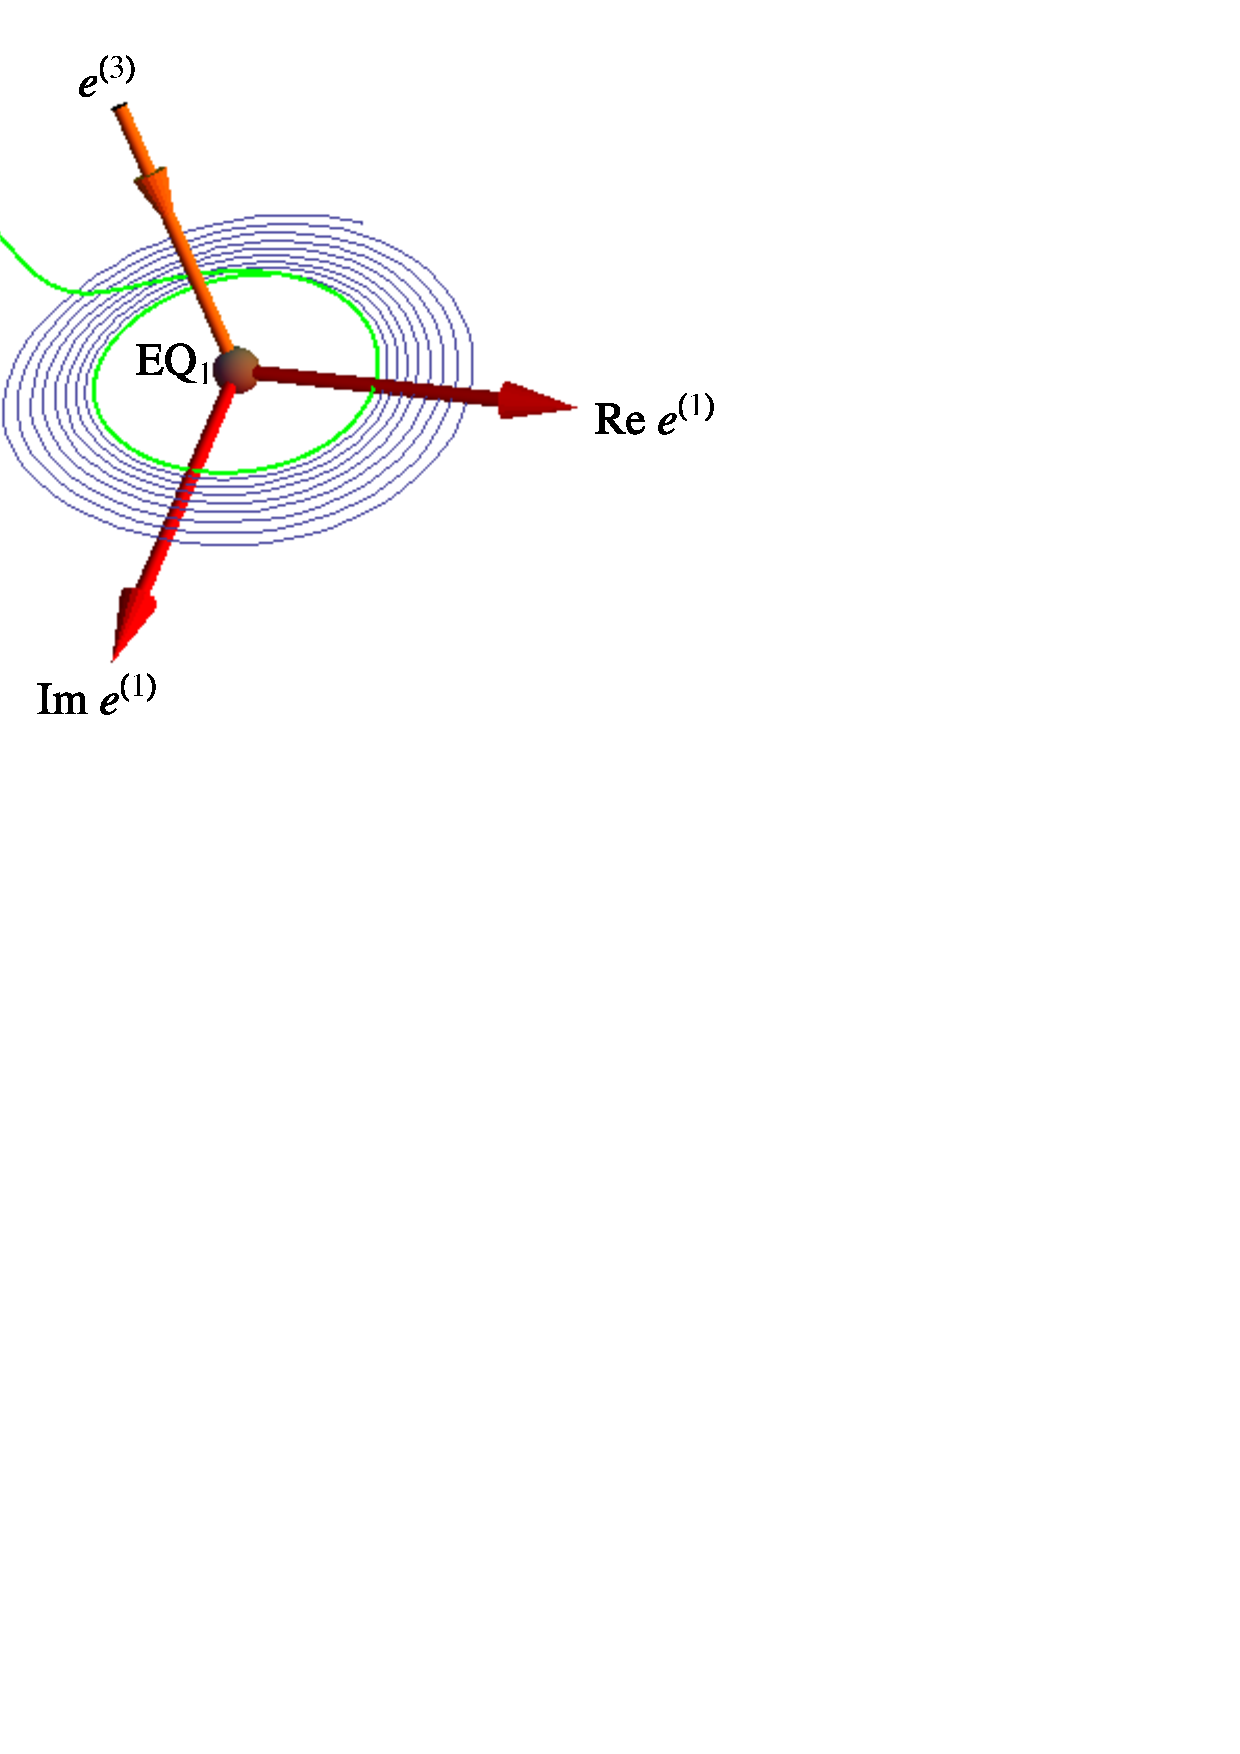
\includegraphics[width=0.36\textwidth]{../Fig/lorenzPolarManifDetail1}  %.png}
(b)  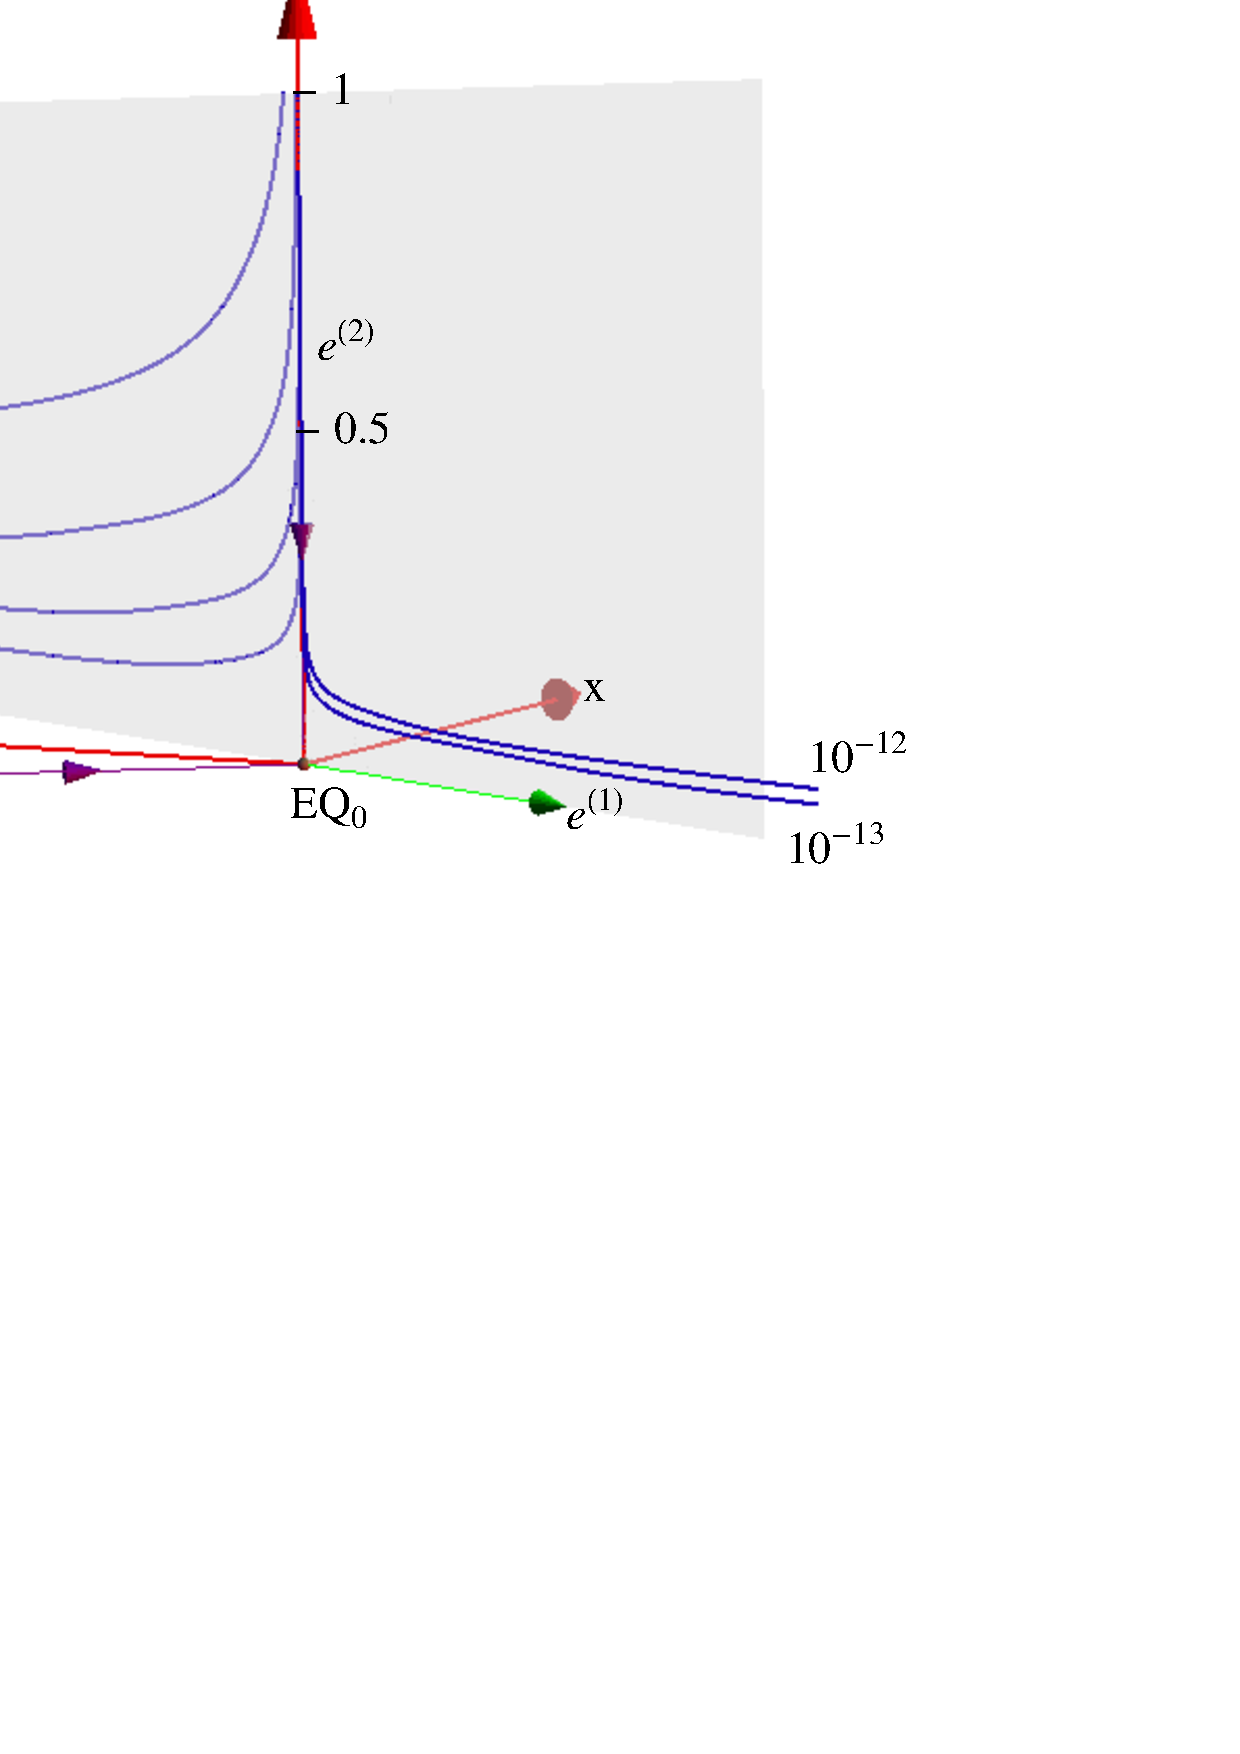
\includegraphics[width=0.56\textwidth]{../Fig/lorenzSaddle0}  %.png}
}{}{
(a) A perspective view of the linearized Lorenz flow near $\EQV{1}$ \eqv,
see \reffig{fig:LorenzSect}\,(a).
The unstable eigenplane of $\EQV{1}$ is
spanned by \Re\jEigvec[1]\ and \Im\jEigvec[1]. The
stable eigen\-vector  $\jEigvec[3]$.
(b) Lorenz flow near the $\EQV{0}$ \eqv: unstable
eigen\-vector  $\jEigvec[1]$,
stable eigen\-vectors  $\jEigvec[2]$,  $\jEigvec[3]$.
Trajectories initiated at distances
$10^{-8}$ $\cdots$ $10^{-12}$, $10^{-13}$ away from the
$z$-axis exit finite distance from $\EQV{0}$  along the
$(\jEigvec[1],\jEigvec[2])$ eigen\-vectors plane.
%starting at approximate from the heteroclinic connection from
%$\EQV{1}$ to $\EQV{0}$.
Due to the strong $\eigExp[1]$ expansion, the
$\EQV{0}$ \eqv\ is, for all practical purposes,
unreachable, and the  $\EQV{1} \to \EQV{0}$ heteroclinic connection
never observed in simulations such as
\reffig{LorenzAttrct}.
(E. Siminos; continued in \reffig{fig:PoincLorenz}.)
    }{fig:LorenzEQ1} %fig:LorenzEQ0}
%%%%%%%%%%%%%%%%%%%%%%%%%%%%%%%%%%%%%%%%%%%%%%%%%%%%%

As all numerical plots of the Lorenz flow are
here carried out for the Lorenz parameter choice
\(
    \sigma = 10, b= 8/3, \rho = 28
\,,
\)
we note the values of these eigenvalues for future reference,
\beq
\barr{lcrl}
\EQV{0}:~
(\eigExp[1],\eigExp[2], \eigExp[3])
    &=& (\,11.83\,,~-2.666,& -22.83\,)   \\
\EQV{1}:~
(\eigRe[1] \pm\,i\,\eigIm[1],\eigExp[3])
    &=& (\,\,0.094\,\pm i\,10.19,\,& -13.85\,) \,, \\
\earr
\label{EqLorenzStab}
\eeq
as
well as the rotation period
$T_{\EQV{1}} = 2\pi/\eigIm[1]$ about $\EQV{1}$,
and the  associated expansion/contraction multipliers
$\ExpaEig^{(i)} = \exp(\eigRe[j] T_{\EQV{1}})$
per a spiral-out turn:
\index{turnover time}
\index{time!turnover}
\beq
T_{\EQV{1}} =  0.6163 \,, \qquad
(\ExpaEig^{(1)},\ExpaEig^{(3)})
   = (\,1.060 \,, 1.957\times 10^{-4} \,)
\,.
\label{EqLorenzMltp}
\eeq
We learn that the typical turnover time scale in this problem is
of order $T \approx T_{\EQV{1}} \approx 1$
(and not, let us say, 1000, or $10^{-2}$). Combined with
the contraction rate \refeq{trA-Lorenz}, this tells us that
the Lorenz flow strongly contracts \statesp\ volumes, by factor of
$ \approx 10^{-4}$ per mean turnover time.

In the $\EQV{1}$ neighborhood the unstable manifold
trajectories slowly spiral out, with
very small radial  per-turn expansion multiplier
$\ExpaEig^{(1)} \simeq  1.06$,
and very strong contraction multiplier
$\ExpaEig^{(3)}  \simeq 10^{-4}$
onto the unstable manifold,
\reffig{fig:LorenzEQ1}\,(a).
This contraction confines, for all practical purposes,
the Lorenz attractor to a 2\dmn\ surface
evident in the section \reffig{fig:LorenzSect}.
    \PC{ChaosBook: develop this text from steady.tex:
        ``For an unstable complex pair $\eigExp[n,n+1]$ of \eqv\ $\EQV{}$,
let $Wmnfld{u (n,n+1)}{EQ}$ denote the orbit of a {circle}
 of infinitesimal radius in the plane about \EQV{}\ spanned
by $\jEigvec[n]_{r}, \jEigvec[n]_{i}$.
This part of the \EQV{}\ unstable manifold is 2\dmn;
its shape can be traced out by computing a set of trajectories with initial
conditions
$\EQV{} + \epsilon (\jEigvec[n]_{r} \cos \theta + \jEigvec[n]_{i} \sin \theta)$
for a set of values of $\theta$.
%In practice, one obtains a more uniform
%distribution of trajectories by setting initial conditions along the line
%$\uEQ + \epsilon \, \bv_{r}^{(n)}$, for a set of values of $\epsilon$.
        }
\PC{remember to delete   {halcrow/Fig/hyperb.*} ??}

%The unstable eigenplane is defined by eigen\-vectors
%$ \Re\jEigvec[2]=(-0.4955, -0.2010, -0.8450)
%  \Im\jEigvec[2]=(0.5325, -0.8464, 0) $
%along the stable eigen\-vector of $\EQV{1}$, $(0.8557, -0.3298, -0.3988) $.

In the $\ssp_{\EQV{0}} = (0,0,0)$ \eqv\ neighborhood the extremely strong
$\eigExp[3] \simeq -23$ contraction along the $\jEigvec[3]$ direction
confines the hyperbolic dynamics near $\EQV{0}$ to the plane
spanned by the unstable eigen\-vector $\jEigvec[1]$,
with $\eigExp[1] \simeq 12$, and
the slowest contraction rate eigen\-vector $\jEigvec[2]$
along the $z$-axis, with $\eigExp[2] \simeq - 3$.
In this plane the strong expansion % $\eigExp[1] \simeq 18$ % JFG: 12?
along $\jEigvec[1]$ overwhelms the
slow  $\eigExp[2] \simeq - 3$ contraction down the $z$-axis,
making it extremely unlikely for a random trajectory
to approach $\EQV{0}$, \reffig{fig:LorenzEQ1}\,(b).
Thus linearization suffices to describe analytically the singular
dip in the Poincar\'e sections of
\reffig{fig:LorenzSect}, and the empirical scarcity
of trajectories close to $\EQV{0}$.
(continued in \refexam{exmp:LorenzContr}.)

\hfill   (E. Siminos and J. Halcrow)
    } %end \example{exmp:LorenzStab


%%%%%%%%%%%%%%%%%%%%%%%%%%%%%%%%%%%%%%%%%%%%%%%%%%%%%%%%%%%%%%%%%%%%%%%%%%
\example{Lorenz flow: Global portrait.}{ \label{exmp:LorenzGlob}
% Predrag                           04apr2008
% Predrag                           19jan2008
% moved to here from halcrow/blog/TEX/lorenz.tex
\index{Lorenz flow}
(continued from \refexam{exmp:LorenzStab}.)
As the $\EQV{1}$ unstable manifold spirals out,
the strip that starts out in the section above $\EQV{1}$
in \reffig{fig:LorenzSect} cuts across the
$z$-axis invariant subspace. This strip necessarily contains a
heteroclinic orbit that hits the $z$-axis
head on, and in infinite time (but exponentially
fast) descends all the way to $\EQV{0}$.
\PC{This needs more explaining. As
    $\EQV{0}$ has 2 contracting dimensions (and fluids will
    have 50,000), whole volumes get scrunched into $\EQV{0}$,
    not just 1\dmn\ heteroclinic orbits.
   }


How? As in the neighborhood of the
$\EQV{0}$ \eqv\ the dynamics is linear
(see \reffig{fig:LorenzEQ1}\,(a)), there
is no need to integrate numerically the final segment
of the heteroclinic
connection - it is sufficient to bring a trajectory
a small distance away from $\EQV{0}$, continue
analytically to a small distance
beyond $\EQV{0}$,
then resume the numerical integration.

What happens next? Trajectories to the left of $z$-axis shoot
off along the $\jEigvec[1]$ direction, and those to the
right along $-\jEigvec[1]$. As along the $\jEigvec[1]$ direction
$xy >0$, the nonlinear term in the $\dot{z}$ equation \refeq{Lorenz}
bends both branches of the
$\EQV{0}$ unstable manifold $W^u(\EQV{0})$ upwards.
Then $\ldots$ - never mind.
Best to postpone the completion of this narrative to
\refexam{exmp:LorenzD1}, where the discrete
symmetry of Lorenz flow will help us streamline the analysis.
As we shall show, what we already know about the 3 \eqva\ and
their stable/unstable manifolds suffices to completely pin down
the topology of Lorenz flow.
(continued in \refexam{exmp:LorenzD1}.)

\hfill   (E. Siminos and J. Halcrow)
    } %end \example{exmp:LorenzGlob


\example{Lorenz flow \statesp\ contraction:}{ \label{exmp:LorenzContr}
\index{Lorenz flow}
(continued from \refexam{exmp:LorenzStab}.)~~
It follows from \refeq{RossLinrz} and \refeq{traceA} that
Lorenz flow is volume contracting,
\beq
\pde_i \pVeloc_i
 = \sum_{i=1}^{3} \eigExp[i](\ssp,t)
= -\sigma -b -1
    \,,
\ee{trA-Lorenz}
at a constant, coordinate- and $\rho$-independent rate, set by
Lorenz to $\pde_i \pVeloc_i = -13.66$ . As for \po s and for
long time averages there is no contraction/expansion along the
flow, $\eigExp[\parallel]=0$, and the sum of $\eigExp[i]$ is
constant by \refeq{trA-Lorenz}, there is only one independent
exponent $\eigExp[i]$ to compute.
~~(continued in \refexam{exmp:LorenzGlob}.)
    } %end example{R\"ossler flow

%from ChaosBook.org \Chapter{discrete}{5sep2008}{World in a mirror}

\example{Equivariance of the Lorenz flow.}{\label{exmp:3dinvDscr}
(continued from \refexam{exmp:3dCoordDscr})
The vector field in Lorenz equations  \refeq{Lorenz} is
equivariant under the action of  cyclic group
$\Ztwo = \{e,\Rot{1/2}\}$
acting on \Rls{3}\ by a $\pi$ rotation about the $z$ axis,
\[
    \Rot{1/2}(x,y,z) = (-x,-y,z)\,.
\]
%This transformation can be considered as either as rotation by
%$\pi$ around the $z$ axis (hence the group \Ztwo) or as a
%reflection about the origin in a plane perpendicular to the
%$z$-axis (hence the group \Dn{1}.)
\index{Lorenz flow!symmetry}
(continued in \refexam{exmp:LorenzD1}.)
        } %end \example{Discrete symmetries of $3d$ flow

%%%%%%%%%%%%%%%%%%%%%%%%%%%%%%%%%%%%%%%%%%%%%%%%%%%%%%%%%%%%%%%%%%%%%%%%%%
\example{Desymmetrization of Lorenz flow:}{ \label{exmp:LorenzD1}
% Predrag                           04apr2008
% Predrag                           19jan2008
% moved to here from halcrow/blog/TEX/lorenz.tex
\index{Lorenz flow}
%\PC{ChaosBook: start the discrete.tex example here, link to the intro example in
%    the flow.tex chapter}
(continuation of  \refexam{exmp:3dinvDscr})
%
~~
Lorenz equation \refeq{Lorenz} is invariant under
the action of order-2 group $\Ztwo = \{e,\Rot{1/2}\}$, where
 $\Rot{1/2}$ is $[x,y]$-plane, constant $z$  rotation by $\pi$ about the $z$-axis:
\beq
(x,y,z) \to \Rot{1/2}(x,y,z) = (-x,-y,z) \,.
\ee{LorenzR}
$(\Rot{1/2})^2=1$ condition decomposes the \statesp\ into two
linearly irreducible subspaces
$\pS = \pS^+ \oplus \pS^-$,
the $z$-axis $\pS^+$ and
the $[x,y]$ plane $\pS^-$, with
projection operators onto the two subspaces given by
(see \refsect{s:ProjOper})
 \beq
 \PP^+ = \frac{1}{2}(1 + \Rot{1/2})
 =   \left(\barr{ccc}
    0  &  0 & 0  \\
    0  &  0 & 0 \\
    0  &  0 & 1
    \earr\right)
     ,\quad
 \PP^- = \frac{1}{2}(1 - \Rot{1/2})
  =   \left(\barr{ccc}
    1  &  0 & 0  \\
    0  &  1 & 0 \\
    0  &  0 & 0
    \earr\right)
\,.
 \label{projOp:sig}
 \eeq
As the flow is $\Ztwo$-invariant, so is its linearization
$\dot{\ssp} = \Mvar \ssp$. Evaluated at $\EQV{0}$, $\Mvar$
commutes with  $\Rot{1/2}$, and,
as we have already seen in  \refexam{exmp:LorenzStab},
the $\EQV{0}$ {\stabmat}
decomposes into $[x,y]$ and $z$ blocks.

The 1\dmn\ $\pS^+$ subspace is
the fixed-point subspace of $\Ztwo$, with the $z$-axis
points left \emph{point-wise} invariant under the group
action
\beq
\mbox{Fix}(\Ztwo) =
   \{ \ssp \in \pS^+ : \mathbf{g} \, \ssp = \ssp \mbox{ for } g \in \{e,\Rot{1/2}\} \}
\,.
\ee{dscr:LorFPsubsp}
\PC{link to definitions in discrete.tex}
However, a point $\ssp(t)$ in $\mbox{Fix}(G)$ moves with time,
but remains within $\ssp(t) \subseteq \mbox{Fix}(G)$ for all
times; the  subspace $\pS^+ = \mbox{Fix}(G)$ is {\em flow
invariant}. In case at hand this jargon is a bit of an
overkill: clearly for $(x,y)=(0,0)$ the full \statesp\ Lorenz
equation \refeq{Lorenz} is reduced to the exponential
contraction to the $\EQV{0}$ \eqv,
\PC{pointer to turbulence chapter here}
\beq
\dot{z} = -b \, z
\,.
\ee{LorenzZaxis}
% which is the reason why you never see this decomposition discussed
% in literature. Even though
However, for flows in higher-dimensional \statesp s the
flow-invariant $\pS^+$ subspace can itself be high-dimensional, with
interesting dynamics of its own.
Even in this simple case this subspace plays an important role
as a topological obstruction, with
the number of winds of a trajectory around it providing
a natural symbolic dynamics.

The $\pS^-$ subspace is, however, {\em not} flow-invariant, as the nonlinear
terms $\dot{z}=xy - bz$ in the Lorenz equation \refeq{Lorenz}
send all initial conditions within
$\pS^-=(x(0),y(0),0)$ into the full, $z(t) \neq 0$ \statesp\  $\pS$.
The $\Rot{1/2}$ symmetry is nevertheless very useful.

By taking as a Poincar\'e section % $\PoincS$
any  $\Rot{1/2}$-invariant, infinite-extent, non-self-inter\-sect\-ing
surface that contains the
$z$ axis, the \statesp\ is divided into a half-space fundamental
domain $\tilde{\pS}=\pS/\Ztwo$ and its $180^o$ rotation $\Rot{1/2}\tilde{\pS}$.
An example is afforded by the $\PoincS$ plane section of
the Lorenz flow in \reffig{fig:LorenzSect}. Take
the  fundamental domain $\tilde{\pS}$ to be the half-space between the
viewer and $\PoincS$. Then the full Lorenz
flow is captured by re-injecting back into $\tilde{\pS}$
any trajectory that exits it, by a rotation of $\pi$ around the $z$ axis.

%%%%%%%%%%%%%%%%%%%%%%%%%%%%%%%%%%%%%%%%%%%%%%%%%%%%%%%%%%%%%%%%%%
%    \PC{ \reffig{fig:PolarLorenz}\,(a): consistency with
%    GHC07 notation (unstable eigs first) requires relabeling of
%    $\EQV{0}$ eigen\-vectors, following \refeq{EqLorenzStab}.}
%    \ES{fixed, March 2008}
%    for \( \sigma = 10, b= 8/3, \rho = 28\,,\)

\FIG{
(a)~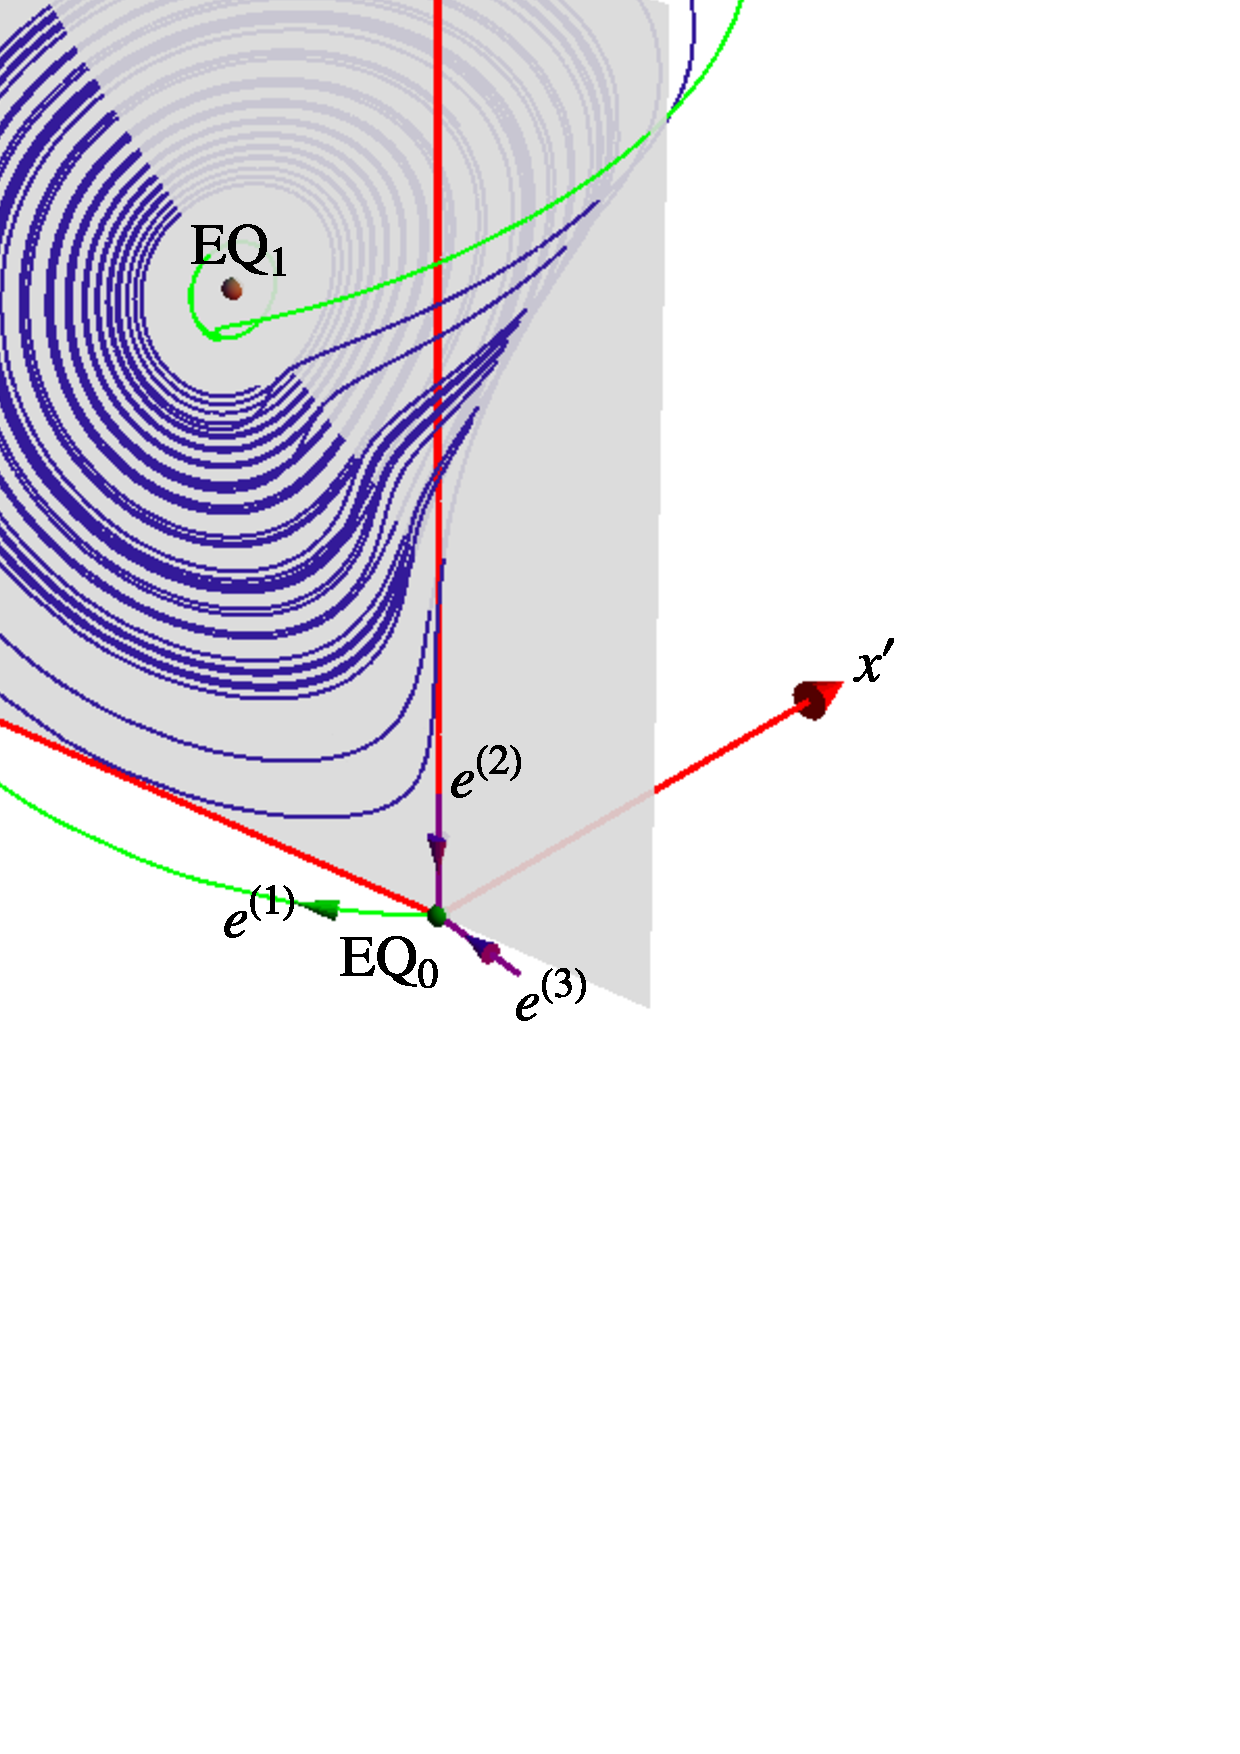
\includegraphics[width=0.40\textwidth]{../Fig/lorenzPolar1}%.png}
~(b)~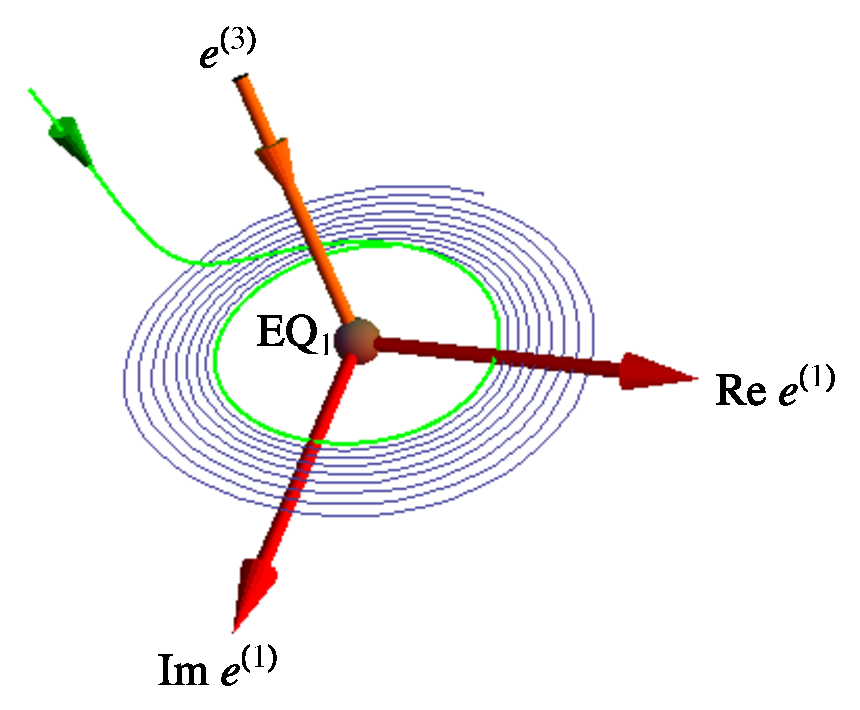
\includegraphics[width=0.44\textwidth]{../Fig/lorenzPolarManifDetail1}
}{}{
(a) % $\Ztwo$-quotiented
Lorenz attractor plotted
in $[x',y',z]$, the doubled-polar angle coordinates \refeq{doubledPolar},
with points related by $\pi$-rotation in the
$[x,y]$ plane identified. Stable eigen\-vectors of $\EQV{0}$:
$\jEigvec[3]$ and $\jEigvec[2]$,
along the $z$ axis \refeq{LorenzZaxis}.
Unstable manifold orbit $W^u(\EQV{0})$
(green) is a continuation of
the unstable $\jEigvec[1]$ of $\EQV{0}$.
(b) Blow-up of the region near $\EQV{1}$:
The unstable eigenplane of $\EQV{1}$ is
defined by $\Re\jEigvec[2]$ and $\Im\jEigvec[2]$, % is shown in red, while
the stable eigen\-vector  $\jEigvec[3]$. % is shown in orange.
The descent of the
$\EQV{0}$ unstable manifold
(green) defines the innermost edge of the strange attractor.
As it is clear from (a), it also defines its outermost edge.
(E. Siminos)
}{fig:PolarLorenz}
%%%%%%%%%%%%%%%%%%%%%%%%%%%%%%%%%%%%%%%%%%%%%%%%%%%%%%%%%%%%%%%%%%


As any such $\Rot{1/2}$-invariant section does the job, a
choice of a `fundamental domain' is here largely mater of
taste. For purposes of visualization it is convenient to make
the double-cover nature of the full \statesp\ by $\tilde{\pS}$
explicit, through any \statesp\ redefinition that maps a pair
of points related by symmetry into a single point. In case at
hand, this can be easily accomplished by expressing $(x,y)$ in
polar coordinates $(x,y) \,=\, (r \cos \theta , r \sin
\theta)$, and then plotting the flow in the
\emph{`doubled-polar angle representation:'}
\beq
(x',y') \,=\, (r \cos 2\theta , r \sin 2\theta)
        \,=\, ( (x^2-y^2)/r, 2xy/r )
\,,
\label{doubledPolar}
\eeq
as in \reffig{fig:PolarLorenz}\,(a). In contract to the
original $G$-equivariant coordinates $[x,y,z]$, the Lorenz flow
expressed in the new coordinates $[x',y',z]$ is {\em
$G$-invariant}, see \refexam{exmp:3dPolyDscr}. In this
representation the $\tilde{\pS}=\pS/\Ztwo$ fundamental domain
flow is a smooth, continuous flow, with  (any choice of) the
fundamental domain stretched out to seamlessly  cover the
entire $[x',y']$ plane.

We emphasize: such nonlinear coordinate transformations are
\emph{not} required to implement the symmetry quotienting
$\pS/G$, unless there are computational gains in a nonlinear
coordinate change suggested by the symmetry. We offer them here
only as a visualization aid that might help the reader
disentangle 2\dmn\ projections of higher-dimensional flows. All
numerical calculations are usually carried in the initial, full
\statesp\ formulation of a flow, with symmetry-related points
identified by \emph{linear} symmetry transformations.
~~(continued in \refexam{exmp:LorenzRetM})

\hfill   (E. Siminos and J. Halcrow)
    } %end Desymmetrization of Lorenz exmp:LorenzD1
%%%%%%%%%%%%%%%%%%%%%%%%%%%%%%%%%%%%%%%%%%%%%%%%%%%%%%%%%%%%%%%%%%%%%%%%%%


%%%%%%%%%%%%%%%%%%%%%%%%%%%%%%%%%%%%%%%%%%%%%%%%%%%%%%%%%%%%%%%%%%%%%%%%%%
\example{\Rpo s of Lorenz flow:}{ \label{exmp:LorenzRpos}
% Predrag                           09feb2009
\index{Lorenz flow}
(continuation of  \refexam{exmp:LorenzD1})
%
The relation between the full \statesp\ periodic orbits,
and the fundamental domain \refeq{doubledPolar} reduced orbits
of the Lorenz flow:
Full \statesp\ cycle pairs $p$, $Rp$ map into
a single cycles $\tilde{p}$ in the fundamental domain, and any
self-dual cycle $p = Rp = \tilde{p}R\tilde{p}$
is a repeat of a \rpo\ $\tilde{p}$.
    } %end Desymmetrization of Lorenz exmp:LorenzD1
%%%%%%%%%%%%%%%%%%%%%%%%%%%%%%%%%%%%%%%%%%%%%%%%%%%%%%%%%%%%%%%%%%%%%%%%%%


%from ChaosBook.org \Chapter{knead}{19feb2009}{Charting the state space}

We start in \refsect{s-symb-dyn} with a simple and intuitive
example, a 3-disk game of pinball. The qualitative dynamics of
stretching/shrinking strips of surviving \statesp\ regions
enables us to partition the {\statesp} and  assign
\emph{symbolic dynamics} itineraries to trajectories. For the
3-disk game of pinball all possible symbol sequences enumerate
all possible orbits.

In \refsect{s:StrtchFld} we use R\"ossler and Lorenz flows to
motivate modeling of higher-dimensional flows by iteration of
1-dimensional maps. For these two flows the 1-dimensional maps
capture essentially all of the higher-dimensional flow
dynamics, both qualitatively and quantitatively. 1-dimensional
maps suffice to explain the two key aspects of qualitative
dynamics; \emph{temporal ordering}, or \emph{itinerary} with
which a trajectory visits \statesp\ regions%
% (\refsect{s-Unimod-symb-dyn})
, and the \emph{spatial ordering}
between trajectory points % (\refsect{s-Spat-ord})%
, which is the
key to determining the admissibility of an orbit with a
prescribed itinerary. In a generic dynamical system not every
symbol sequence is realized as a dynamical trajectory; as one
looks further and further, one discovers more and more rules
which prohibit families of itineraries. For 1-dimensional
\stretchf\ maps the \emph{kneading theory} % (\refsect{s-knead})
provides the definitive answer as to which temporal itineraries
are {\em \admissible} as trajectories of the dynamical system.



{\bf From $d$-dimensional flows to 1-dimensional maps}

Symbolic dynamics for the $3$-disk game of pinball is so
straight\-forward that one may altogether fail to see the
connection between the topology of hyperbolic flows and their
symbolic dynamics. This is brought out more
clearly by the 1-dimensional visualization of \stretchf\ flows
to which we turn now.

So a typical dynamical system
that we care about is {\em bounded}. If the price to keep going
is high - for example, we try to stir up some tar, and observe
it come to a dead stop the moment we cease our labors - the
dynamics tends to settle into a simple state. However,
as the resistance to change decreases - the tar is heated up
and we are more vigorous in our stirring - the dynamics becomes
unstable.



You get the idea - R\"ossler flow winds around the stable manifold of the
`central' \eqv, stretches and folds, and  the
flow can be reduced to a 1-dimensional map. The next example is
similar, but the folding mechanism is very different: the unstable
manifold of one of the \eqva\ collides with the stable manifold
of the other one, forcing a robust {\em heteroclinic
connection} between the two.
    \index{heteroclinic connection}

%
%%%%%%%%%%%%%%%%%%%%%%%%%%%%%%%%%%%%%%%%%%%%%%%%%%%%%
%\PC{figs/lorenzPolarPoinc2.eps was 0.7MB - ES reduced to 14KB.
%    figs/lorenzPolarPoinc1.eps 0.8MB - now not used
\FIG{
(a)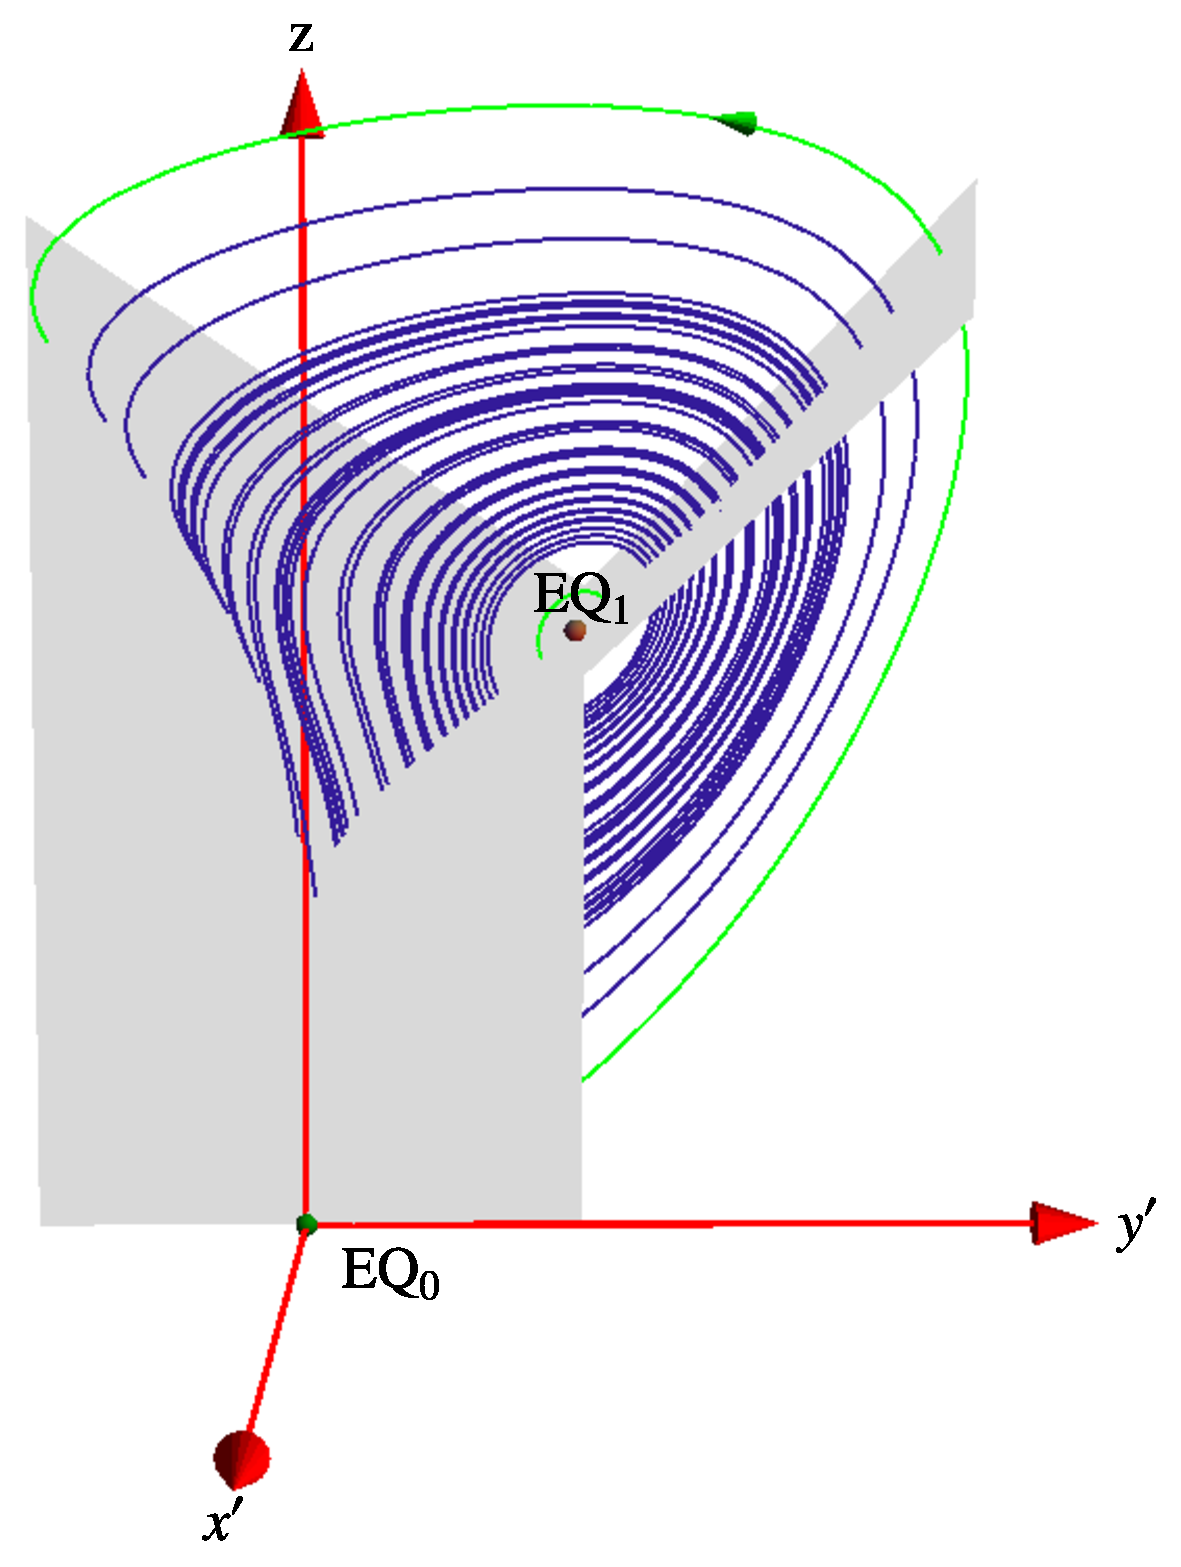
\includegraphics[width=0.42\textwidth]{../Fig/lorenzPolarPoinc2}%
~~%
(b)\raisebox{2.4ex}{
    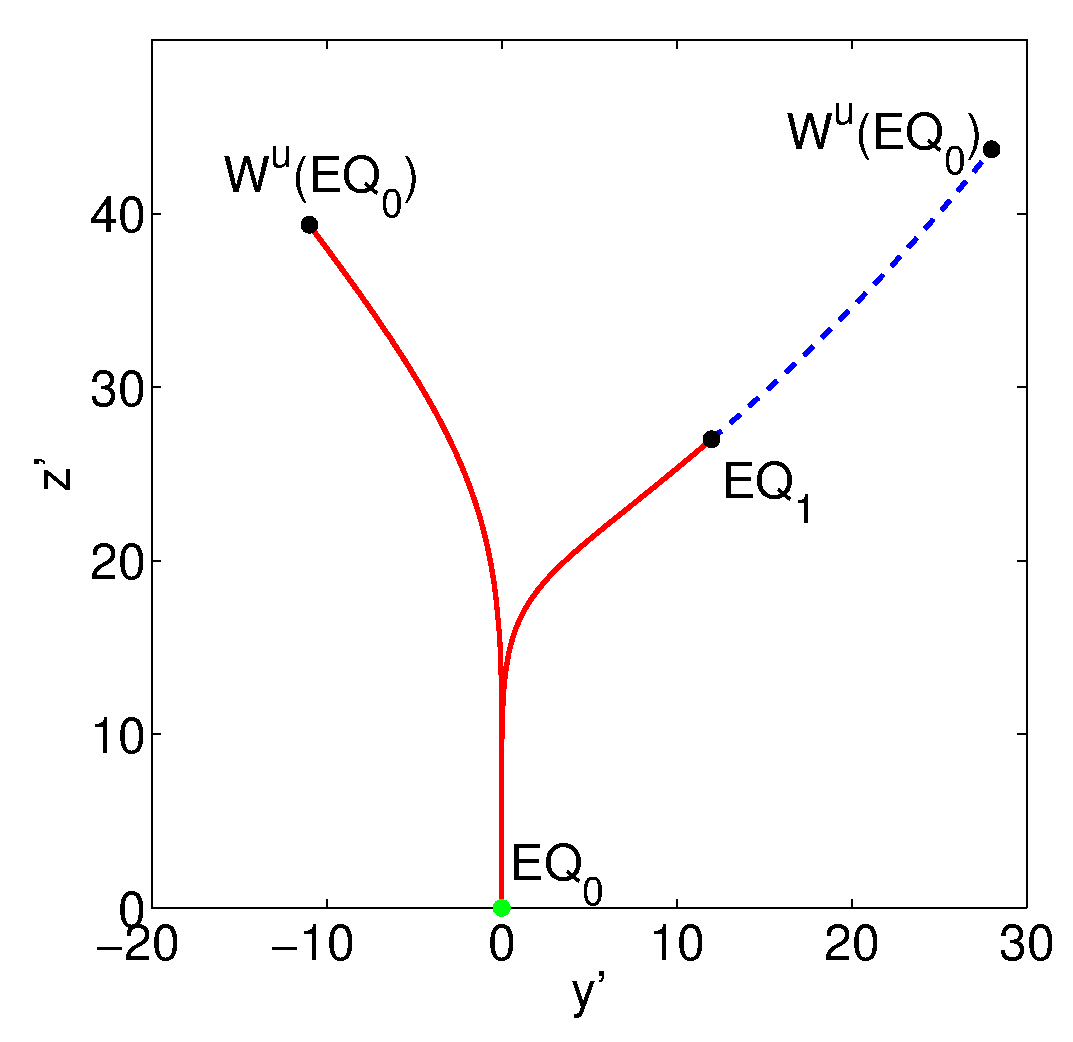
\includegraphics[width=0.44\textwidth]{../Fig/plorenz_psec}
                   }
}{}{
(a) A Poincar\'e section % $\PoincS_1$
of the Lorenz flow
in the doubled-polar angle representation, \reffig{fig:PoincLorenz},
given by the $[y',z]$ plane that contains the $z$-axis and
the \eqv\ $\EQV{1}$.
% Most of the section plane except for the
% two shaded trapezoids is removed to aid visualization of the flow.
$x'$ axis points toward the viewer.
%, with the portion of the flow piercing into
% the  section % $\PoincS_1$ shown.
%(b) The same section rotated by $\pi$ in the $[x',y']$ plane, viewed
%from above. Now the flow exiting the section % $\PoincS_1$
%is shown. This view illustrates
%the sharp folding of the outer branch, with the outermost edge
%given by the unstable manifold of $\EQV{0}$.
(b) The Poincar\'e section of the Lorenz flow by the section %$\PoincS_1$
plane (a); compare with \reffig{fig:LorenzSect}.
Crossings \emph{into} the section
are marked red (solid) and
crossings \emph{out of} the section are marked blue (dashed).
% (green dot) $\EQV{1}$ \eqv.
% (black dot) $\EQV{0}$ at the origin.
Outermost points of both in- and out-sections
are given by the $\EQV{0}$ unstable manifold $W^u(\EQV{0})$
intersections.
(E. Siminos)
}{fig:PoincLorenz}
%%%%%%%%%%%%%%%%%%%%%%%%%%%%%%%%%%%%%%%%%%%%%%%%%%%%%%%%%%%%%%%%%%
%

%%%%%%%%%%%%%%%%%%%%%%%%%%%%%%%%%%%%%%%%%%%%%%%%%%%%%%%%%%%%%%%%%%%%%%%%%%
\example{Lorenz flow:
        Stretch \&\ crease.}{ \label{exmp:LorenzRetM}
% Predrag                           04apr2008
% Predrag                           19jan2008
% moved to here from halcrow/blog/TEX/lorenz.tex
\index{Lorenz flow}
%
%%%%%%%%%%%%%%%%%%%%%%%%%%%%%%%%%%%%%%%%%%%%%%%%%%%%%%%%%%%%%%%%%%
% old {fig:PoincLorenz}\,(d)
\SFIG{plorenz_retmap2}
{}{
The Poincar\'e return map $s_{n+1}=\PoincM(s_n)$ parameterized by
Euclidean arclength $s$ measured along the
$\EQV{1}$ unstable manifold,
from $\ssp_{\EQV{1}}$ to  $W^u(\EQV{0})$ section point,
uppermost right point of the blue segment in
\reffig{fig:PoincLorenz}\,(b).
% PC deal with this:
% \JFGedit{(JFG: ``upper half''? I don't get it, e.g. I don't see
% how (d) is connected to what part of (c))}
The critical point (the `crease') of the map is given by
the section of the heteroclinic orbit $W^s(\EQV{0})$
that descends all the way to
$\EQV{0}$, in infinite time and with infinite slope.
(E. Siminos)
}{fig:RetMapLorenz}
%%%%%%%%%%%%%%%%%%%%%%%%%%%%%%%%%%%%%%%%%%%%%%%%%%%%%%%%%%%%%%%%%%
%
\PC{copy this exercise to an appendix, keep a brief summary here;
    or split int several examples, the first one taken back to
    discrete.tex
    }
We now deploy the symmetry of Lorenz flow
to streamline and complete analysis of the Lorenz strange attractor
commenced in  \refexam{exmp:LorenzD1}. There we showed that
the dihedral $D_1 = \{e,R\}$ symmetry identifies the
two \eqva\ $\EQV{1}$ and $\EQV{2}$,
and the traditional `two-eared' Lorenz flow
\reffig{LorenzAttrct} is replaced by
the `single-eared' \PublicPrivate{}{Van Gogh} flow
of \reffig{fig:PolarLorenz}\,(a).
Furthermore, symmetry identifies two sides of any plane
through the $z$ axis, replacing a full-space Poincar\'e
section plane by a half-plane, and the two directions
of a full-space eigen\-vector of $\EQV{0}$
 by a one-sided eigen\-vector, see \reffig{fig:PolarLorenz}\,(a).

\refExam{exmp:LorenzGlob} explained the genesis of the
$\ssp_{\EQV{1}}$ {\eqv} unstable manifold, its orientation and
thickness, its collision with the $z$-axis, and its
heteroclinic connection to the $\ssp_{\EQV{0}} = (0,\, 0,\, 0)$
{\eqv}. All that remains is to describe how the $\EQV{0}$
neighborhood connects back to the $\EQV{1}$ unstable
manifold. \refFig{fig:PolarLorenz} now shows clearly how the
Lorenz dynamics is pieced together from the 2 \eqva\ and their
unstable manifolds:

Having completed the descent to  $\EQV{0}$, the
infinitesimal neighborhood of the heteroclinic $\EQV{1} \to
\EQV{0}$ trajectory is ejected along the unstable manifold
of $\EQV{0}$ and is re-injected into the unstable manifold
of $\EQV{1}$. Both sides of the narrow strip enclosing the
$\EQV{0}$ unstable manifold  lie above it, and they get
folded onto each other with a knife-edge crease (contracted
exponentially for infinite time to the  $\EQV{0}$
heteroclinic point), with the heteroclinic out-trajectory
defining the outer edge of the strange attractor. This leads to
the folding of the outer branch of the Lorenz strange
attractor, illustrated in \reffig{fig:PoincLorenz}\,(b), with
the outermost edge following the unstable manifold of
$\EQV{0}$.

Now the stage is set for construction of  Poincar\'e sections
and associated  Poincar\'e return maps. There are two natural
choices; the section at $\EQV{0}$, lower part of
\reffig{fig:PoincLorenz}\,(b), and the section (blue) above
$\EQV{1}$. The first section, together with the blowup of
the $\EQV{0}$ neighborhood, \reffig{fig:LorenzEQ1}\,(b),
illustrates clearly the scarcity of trajectories (vanishing
natural measure) in the neighborhood of $\EQV{0}$. The flat
section above $\EQV{1}$ (which is, believe it or not, a
smooth conjugacy by the flow of the knife-sharp section at
$\EQV{0}$) is more convenient for our purposes. Its return
map  \refeq{orientCond} is given by \reffig{fig:RetMapLorenz}.

The rest is straight sailing: to accuracy $10^{-4}$ the return
map is unimodal, its critical point's forward trajectory
yields the \ks\ \refeq{e_kappa_def}, and the \admissible\ binary
sequences, so any number of periodic points  can be accurately
determined from this 1-dimensional return map, and the 3\dmn\
cycles then verified by integrating the Lorenz differential
equations \refeq{Lorenz}. The map is everywhere expanding on
the strange attractor, so it is no wonder mathematicians can
here make the ergodicity rigorous.
    \PC{Paragraph here - codimensionality of manifolds from
        paper with Viswanath}

% (continued in \refexam{exmp:Lorenz??})
\hfill   (E. Siminos and J. Halcrow)
    } %end \example{Lorenz flow: a 1\dmn\ return map} exmp:LorenzRetM
%%%%%%%%%%%%%%%%%%%%%%%%%%%%%%%%%%%%%%%%%%%%%%%%%%%%%%%%%%%%%%%

What have we learned from the above two exemplary 3-dimensional
flows? If a flow is locally unstable but globally bounded, any
open ball of initial points will be stretched out and then
folded back. If the \eqva\ are hyperbolic, the trajectories
will be attracted along some eigen-directions and ejected along
others. The unstable manifold of one \eqv\ can avoid stable
manifolds of other \eqva, as is the case for R\"ossler, or
slice them head on, as is the case for Lorenz. Hence
qualitatively a typical trajectory will wander through
\statesp, being alternatively attracted into \eqva\
neighborhoods, and then ejected again. What is important is the
motion along the unstable manifolds --that is where
1-dimensional maps come from.


  \Remarks

\remark{Lorenz equation.}{ \label{rem:Lorenz}
% Predrag                           20jan2008
% transferred from halcrow/thesis/chapters/symm.tex
The Lorenz equation \refeq{Lorenz} is
the most celebrated early
illustration of ``deterministic chaos''\rf{lorenz63}
(but not the first -
the honor goes to Dame Cartwright\rf{disc:CarLit45}).
Lorenz's paper, which can be found in reprint
collections \refrefs{cvt89b,hao90b}, is a pleasure to read, and
is still one of the best introductions to the physics
motivating such models.
For a geophysics derivation, see Rothman course notes\rf{Rothman06}.
The equations, a set of ODEs in $\reals^3$, exhibit strange
attractors\rf{tucker1,tucker2,MIViana}.
% whose geometry reflects
%the underlying symmetry of the ODEs.
Fr{\o}yland\rf{froyland} has a nice brief discussion
of Lorenz flow.
Fr{\o}yland and Alfsen\rf{froyland_alfsen} plot
many periodic and heteroclinic orbits of the Lorenz flow;
some of the symmetric ones are included in \refref{froyland}.
Guckenheimer-Williams\rf{Guckenheimer79b} and
Afraimovich-Bykov-Shilnikov\rf{Afraimovich87} offer
in-depth discussion of the Lorenz equation.
The most detailed study of the Lorenz equation
was undertaken by Sparrow\rf{sparrow}.
For a physical interpretation of $\rho$ as ``Rayleigh number.''
see Jackson\rf{jackson89} and Seydel\rf{seydel}.
Lorenz truncation to 3 modes is
so drastic that the model bears no relation to  the physical
hydrodynamics problem that motivated it.
For a detailed pictures of Lorenz invariant manifolds consult
 Vol II of Jackson\rf{jackson89}.
Lorenz attractor is a very thin fractal -- as we saw,
stable manifold thinckness is of order $10^{-4}$ -- but its
fractal structure has been accurately resolved by
D. Viswanath\rf{Viswanath03,Viswanath04}.
\hfill (continued in \refrem{rem:LorenzSymm}.)
    } %end \remark{Lorenz equation:}{ \label{rem:Lorenz}

\remark{H\'enon, Lozi maps.}{
%chaos.nbi.dk:/users/predrag/nordita/tex/henon_long/henon.tex
%      PC                  10/5-94
The H\'enon map%\rf{henon}
\index{Henon@H\'enon map}
% {\em per se}
is of no particular physical
import in and of itself--its significance lies in
the fact that it is a minimal normal form for modeling flows near a
\snbif,
\index{bifurcation!saddle-node}
\index{saddle-node bifurcation}
and that it is a prototype of the stretching and folding dynamics that
leads to deterministic chaos.  It is generic in the sense that it can
exhibit arbitrarily complicated symbolic dynamics and mixtures of
hyperbolic and non--hyperbolic behaviors.  Its construction was
motivated by the best known early example of `deterministic chaos',
the Lorenz equation\rf{lorenz}, see \refref{lorenz}
and \refrem{rem:Lorenz}.

\index{Lorenz, E.N.}
\index{Pomeau, Y.}
 Y.~Pomeau's studies of the Lorenz
attractor on an analog computer, and his insights into its stretching
and folding dynamics motivated H\'enon\rf{henon} to introduce
the H\'enon map in
1976.
\index{Henon@H\'enon, M.}
H\'enon's and Lorenz's original papers can be found in reprint
collections \refrefs{u_in_c,hao}.  They are a pleasure to read, and
are still the best introduction to the physics
%background
motivating such models.
A detailed description of the dynamics of the H\'enon map is
given by Mira and coworkers\rf{mira}, as well as very many other
authors.
\index{Mira, C.}
% Mira and coworkers\rf{fou,mira}, as well as very many
% other\rf{AP,AGIP,BC85,BC89,BC91,biham_wenzel_89,biham_wenzel_90,
% losal,CGP,GK85,GKM,GK85,hansen_henon,henon,milnor,mira,simo}.

\index{Lozi map}
\index{map!Lozi}
The Lozi map\rf{lozi2} is particularly convenient in investigating the
symbolic dynamics of $2\dmn$ mappings.  Both the Lorenz and Lozi
systems are uniformly smooth systems with singularities.
The continuity of measure
for the Lozi map
was proven by M.~Misiurewicz\rf{mis1},
and the existence of the SRB measure was established by L.-S.~Young.
% \index{SRB measure}  is in indexPointers.tex
\index{natural measure}
\index{measure!natural}
\index{Misiurewicz, M.}
\index{Young, L.-S.}
} %end \remark{H\'enon map?}{

\remark{\protect Grasshoppers {\em vs.} butterflies.}{%
\index{sensitivity to initial conditions}
\index{butterfly effect}
The 'sensitivity to initial conditions' was
discussed by Maxwell, 30 years later by Poincar\'e.
In weather prediction, the
Lorentz' `Butterfly Effect' started its journey in
1898, as a `Grasshopper Effect' in a book review by
W. S. Franklin\rf{Frank1898}.  In 1963 Lorenz
ascribed a `seagull effect' to an unnamed meteorologist,
and in 1972 he repackaged it as the `Butterfly Effect'.
           } % \remark{

% Predrag  27mar2008: returned from Halcrow blog to discrete.tex \refref{CEsym}.
% Predrag  20jan2008: moved to Halcrow blog
%
\remark{Symmetries of the Lorenz equation:}{ \label{rem:LorenzSymm}
(continued from \refrem{rem:Lorenz}.)
After having studied  \refexam{exmp:LorenzD1}
you will appreciate why {\tt ChaosBook.org}
starts out with the  symmetry-less
R\"ossler flow \refeq{Roesl_eq}, instead of the
better known Lorenz flow \refeq{Lorenz}
(indeed, getting rid of symmetry
was one of R\"ossler's motivations).
He threw the baby out with the water; for Lorenz flow
dimensionalities of stable/unstable manifolds
make possible a
robust heteroclinic connection absent from R\"ossler flow,
with unstable manifolds of an \eqv\ flowing into the
stable manifold of another \eqva.
How such connections are forced upon us is
best grasped by perusing the chapter 13 `Heteroclinic tangles'
of the inimitable
Abraham and Shaw illustrated classic\rf{abraham:shaw}.
Their beautiful hand-drawn sketches elucidate the origin
of heteroclinic connections in the Lorenz flow (and its high-dimensional
Navier-Stokes relatives) better than any computer simulation.
Miranda and Stone\rf{GL-Mir93} were first to
quotient the $\Ztwo$ symmetry and explicitly construct
the desymmetrized, `proto-Lorenz system,'
by a nonlinear coordinate transformation into the Hilbert-Weyl
polynomial basis
invariant under the action of the symmetry group%
\rf{CoLiSh96}.
For in-depth discussion of symmetry-reduced (`images')
and symmetry-extended (`covers')
topology, symbolic dynamics, periodic orbits,
invariant polynomial bases \etc, of
Lorenz, R\"ossler and many other low-dimensional systems
there is
no better reference than the
Gilmore and Letellier monograph\rf{GL-Gil07b,GL-Let01}.
%
They interpret the proto-Lorenz and its `double
cover' Lorenz as `intensities' being
the squares of `amplitudes,' and call quotiented
flows such as (Lorenz)/$\Ztwo$ `images.'
Our `doubled-polar angle' visualization
\reffig{fig:PoincLorenz}
is a proto-Lorenz in disguise, with the difference: we
integrate the flow and construct Poincar\'e sections and
return maps in the Lorenz $[x,y,z]$ coordinates, without
any nonlinear coordinate transformations.
The Poincar\'e
return map \reffig{fig:RetMapLorenz} is reminiscent
in shape both of the one given by Lorenz
in his original paper, and the one plotted in
a radial coordinate by Gilmore and Letellier.
Nevertheless, it is profoundly different:
our return maps are
from unstable manifold $\to$ itself\rf{CCP96},
and thus intrinsic and coordinate independent. This is necessary
in high-dimensional flows
to avoid problems such as double-valuedness of return map projections
on arbitrary 1\dmn\ coordinates encountered already in
the R\"ossler example. More importantly, as we know the embedding
of the unstable manifold into the full \statesp, a periodic point
of our return map \emph{is} - regardless of the
length of the cycle -  the periodic point in the full  \statesp,
so no additional Newton searches are needed.
\PC{ChaosBook: link this to the figures}

\index{Lorenz, E.N.}
\index{Cartwright, M.L.}
\index{Gilmore, R.}
\index{Letellier, C.}
    } %end \remark{Lorenz equation:}{ \label{rem:LorenzSymm}


\remark{Examples of systems with discrete symmetries.}{
One has
a $\Ztwo$ symmetry in the Lorenz system (\refrem{rem:Lorenz}), % \rf{lorenz,GO},
the Ising model,
and in the 3\dmn\ anisotropic Kepler
potential\rf{gut82,TW,CC92},
a $D_3=\Zn{3v}$ symmetry in H\'enon-Heiles type potentials\rf{HH,JS,rich,laur},
a $D_4=\Zn{4v}$ symmetry in quartic oscillators\rf{EHP,MWR},
in the pure $x^2 y^2$ potential\rf{Mat,CP} and
in hydrogen in a magnetic field\rf{EW1},
and a $D_2=\Zn{2v} = V_4 =\Ztwo\times \Ztwo$ symmetry
in the stadium billiard\rf{robbDisc}.
A very nice application of desymmetrization is
carried out in \refref{BVdisc}.
\index{stadium billiard}\index{billiard!stadium}
\index{Ising model}
        }

    \PublicPrivate{
    }{ % switch \PublicPrivate{
\remark{Nomenclature.}{
Cite Huygens, Poincar\'e for \reqva.
Remember to mention the Lorenz kind of `image' discussed by
Gilmore and Letellier\rf{GL-Gil07b}: if $z$ belongs to the symmetry
invariant $\mbox{Fix}(G)$ subspace, one can replace dynamics in the
full space by $\dot{z}$, $\ddot{z}$, $\cdots$. That is
$G$-invariant by construction.
\PCedit{Replace `desymmetrized {\statesp}' by
    `orbit space?' `image space?'}
Cite literature that uses
`desymmetrized space,'
`image space,'
`orbit space,'
`quotient space.'
} %end \remark{Nomenclature

\remark{Literature.}{
For a summary of discrete groups see \refref{stevenj}.
\PC{Idea: a conserved quantity $\to$ continuous symmetry.
    Can one use Noether theorem?
    }
Chapter 3 of Rebecca Hoyle\rf{hoyll06} is a very
student-friendly overview of all of the group theory
a nonlinear dynamicist might need, with exception of
quotienting, reduction of dynamics to fundamental domains
which is not discussed at all. Curiously, we have not read any of the
group theory books that she recommends as background reading,
which just confirms that there are too many group theory books in all.
For example, one that you will not find useful at all is
\refref{GroupThe}. The reason is presumably that in physics (where
much of the modern group theory was first formulated)
the focus is on the linear representations used in
quantum mechanics, crystallography and quantum field theory.
We shall need these techniques in
\refChap{c-symm} where we reduce the
linear action of evolution operators to irreducible subspaces.
However, here we are looking at nonlinear dynamics, and the
emphasis is on the symmetries of orbits, their isotropy-group
reductions, and the isotypic decomposition of their linear
stability matrices.

Chapter 4 of Rebecca Hoyle\rf{hoyll06} is a
student-friendly introduction
to the treatment of bifurcations in presence of symmetries
worked out in full detail and generality in monographs by
Golubitsky, Stewart and Schaeffer\rf{golubII},
Golubitsky and Stewart\rf{golubitsky2002sp} and
Chossat and Lauterbach\rf{ChossLaut00}.

Amazon.com reviewers rave about \refref{ITO96};
looks nice, get it.
Check out
 \refrefs{ChePiWa02,Jaco05,Kett95,Hall67}.
    } %end\remark{Literature}{
    } % end \PublicPrivate{

    \PublicPrivate{
    }{ % switch \PublicPrivate{
\remark{Literature}{
A summary of discrete groups\rf{stevenj}.
\PC{Idea: a conserved quantity $\to$ continuous symmetry.
    Can one use Noether theorem?
\ESedit{ES: I think that we unfortunatelly cannot use it for dissipative
  systems. Noether's theorem applies provided
  we can formulate the system as a variational problem. It has caused
  me a great deal of confusion tending to think of symmetries in
  this noetherian way even for dissipative systems.
  Some recent progress(?) beyond Noether's theorem is summarized in \href{http://arxiv.org/abs/math-ph/0511035}{\url{math-ph/0511035}}.
  }

    }

Amazon.com reviewers rave about \refref{ITO96}.

Check out \refref{ITO96} (looks nice, get it)
and
 \refrefs{ChePiWa02,Jaco05,Kett95,Hall67}.

% A book(but elementary, not useful):
% http://www.sst.ph.ic.ac.uk/people/d.vvedensky/courses.html

I like a lot Ian Melbourne's work on
 \href{http://personal.maths.surrey.ac.uk/st/I.Melbourne/symmetric_attractors.html}{symmetric attractors}.
I find the distinction between instantaneous symmetry and symmetry
on average very meaningful and potentially useful for us (it will appear
in the thesis soon.)

    } %end\remark{Literature}{
    } % end \PublicPrivate{

\remark{A brief history of relativity:}{
The relative equilibria and relative periodic solutions
are related to
equilibria and periodic solutions respectively
of the Hamiltonian reduced by the symmetries.
They appear in many physical situations,
such as motion of rigid bodies, gravitational
$N$-body problems, molecules and nonlinear waves.
Chenciner\rf{AlbChe98,Chenc03} says
the first attempt to find (relative) periodic solutions of the
$N$-body problem by
was the 1896 short note by Poincar\'e\rf{Poinc1896},
in the context of the 3-body problem.
\Reqva\ of the $N$-body problem
(known in this context as the Lagrange points, stationary in
the co-rotating frame) are circular motions in the inertial frame,
and {\rpo s} correspond to quasiperiodic motions in the inertial frame.
In the planar $N$-body problem the equations are unchanged by
rotations. \Reqva\ can exist in a rotating frame,
and are called central configurations.
For \rpo s in celestial mechanics see also \refref{Broucke75}.
However, according to
Cushman, Bates\rf{CushBat97} and Yoder\rf{Yode88},
C. Huygens\rf{Huyg1673} understood the \reqva\ of a
spherical pendulum many
years before publishing them in 1673.

Lan has some relative equilibria (traveling waves) for KS in his
thesis\rf{Lan:Thesis}, %http://chaosbook.org/projects/theses.html
 and for complex LG in a paper on ``MAWs.''
Viswanath\rf{ViswanathPC06} % arXiv.org/physics/0604062
found them in the plane Couette problem.
Siminos and Davidchack have for box size $L=22$ some equilibria.
Striking application of \rpo s has been the discovery
of ``choreographies" of $N$-body problems%
\rf{CheMon00,CGMS02,McCordMontaldi}.

\label{cont:rpoCond}
} %end \remark{A brief history of relativity:}{

\remark{Stability ordering.}{
The stability ordering was introduced by
Dahlqvist and Russberg\rf{DR91} in a study of chaotic dynamics for the
$(x^2y^2)^{1/a}$ potential.
%in the quantum case.
The presentation here runs along the lines of
Dettmann and Morriss\rf{DM97} for the Lorentz gas
which is hyperbolic but the symbolic dynamics is highly pruned, and
Dettmann and Cvitanovi\'c\rf{DC98} for a family of intermittent maps.
In
%all of
the
%above
applications discussed in the above papers, the stability ordering
yields a considerable improvement over the topological length
ordering. In quantum chaos applications cycle expansion cancelations
are affected by the phases of pseudocycles (their actions), hence
{\em period ordering} rather than stability is frequently employed.
                        } %end \remark{Stability ordering

\remark{Surveys of rigorous theory.}{ \label{rem:rig-z}
We recommend the references listed in \refrem{s-GuideLit}
for an introduction to
the mathematical literature on this subject.
For a physicist, Driebe's monograph\rf{Driebe99}
might be the most accessible
introduction into mathematics discussed briefly in this chapter.
There are a number of reviews of the mathematical approach to
\dzeta s and \Fd s, with pointers to the original references,
such as \refrefs{Viv-1,Poll-1}. An alternative approach to spectral
properties of the \FPoper\ is given in \refref{Via-1}.

Ergodic theory, as presented by Sinai\rf{er-sinai} and others,
tempts one to describe the densities on which the \evOper\ acts
in terms of either
integrable or square-integrable functions. For our
purposes, as we have already seen,
this space is not suitable.
An introduction to ergodic theory is given by
Sinai, Kornfeld and Fomin\rf{Korn}; more advanced
old-fashioned  presentations are Walters\rf{Walt82}
and Denker, Grillenberger and Sigmund\rf{DGS76}; and a more formal
one is given by Peterson\rf{Peterson}.
        %\MAP{  Warwick Tucker
W.~Tucker\rf{tucker1,tucker2,MIViana} has proven rigorously via interval
     arithmetic that the Lorentz attractor is strange for
     the original parameters, and has a long stable periodic orbit for
     the slightly different parameters.

} %end \remark{Surveys of rigorous theory}{

\RemarksEnd
